\chapter{General Introduction}
\label{chapter:introduction}
The ideas put forward in this chapter are based in parts on work that I contributed to a review \citep[P2]{Mueller-Hansen2017} and a modeling framework paper \citep[P3]{Donges2018}.
\section{Complex Systems Models to Navigate the Anthropocene}
\label{sec:intro_complex_systems}
% The climate crisis makes rapid societal change necessary.
Over the last centuries, human impacts on Earth's geology and ecosystems have reached unprecedented levels -- to the point where `the Anthropocene', the age of the humans is discussed as a new epoch in geological time \citep{Crutzen2006, Zal2008, Zal2010, Steffen2011}. In this new epoch, the future trajectory of the Earth is governed by Earth system processes on the physical and biological level as well as human processes in economies, societies and culture \citep{Steffen2007, Lewis2015, Crutzen2016}.

The current trajectory in the Anthropocene brings with it a number of substantial challenges for a prosperous life of the human species in the future such as anthropogenic climate change and rapid degeneration of biosphere integrity. In order to sustain the conditions of the Holocene that are essential for the prosperity (in the global north) up to this point, we need to drastically reduce the pressure that we exert on the ecosystems that we depend on and the amount of green house gases that are emitted \citep{Rockstrom2009a, Rockstrom2009, Steffen2015a}.

% Contemporary IAMs have a somewhat simplified view on society and don't picture e.g. social movements
In the face of this, it becomes more and more apparent that in order to stay within the GHG emissions budgets that promise to keep global warming below $1.5^\circ$~C alone, rapid changes in society and economy are necessary \citep{Rockstrom2017, Geels2017}.
To find ways to navigate the possible scenarios for these changes, different, highly sophisticated so called integrated assessment models (IAMs) are in use \citep{VanVuuren2016}.
Most of those models rely on neoclassical economics to describe their societal parts. In most cases, this means that they make very strict assumptions about human motivation, mode of reasoning and cognitive capacities e.g., they generally assume that individuals' primary drive is the consumption of goods and services, which they optimize farsightedly, and that firms' primary objective is to maximize profits. They usually also assume that humans and firms do this in particular ways which allows their plurality to be described as the behavior of one representative individual, respectively.
However, with all the convenience for analysis that comes with this set of assumptions, they pose strong limitations on the possible effects that can be described with a model \citep{Kirman1992}.
Particularly, many inherent properties of economic systems such as cyclic fluctuations in economic output or herding and bubbles in markets emerge from localized interactions between diverse individual agents \citep{Levin1998, Tesfatsion2003, Anderson2018}. As such they cannot be pictured by the neoclassical paradigm that inherently relies on representative agents. 
At the same time, there is ample historical evidence that large scale changes in society and economy such as voting, reproductive, and other rights for women, the abolishment of slavery and equal rights for African Americans or unionization of workers, just to name a few, were the merit of social movements rather than a consequence of changing supply and demand \citep{Tarrow2011, Tilly2019}. 
This poses a challenge to many contemporary models that are used to describe climate change and to explore possible mitigation and adaptation scenarios: how can they model societal changes that are driven by processes of social interaction, opinion formation, changing norms and values and consequential changes in individual decision making?
\begin{figure}[t]
  \centering
  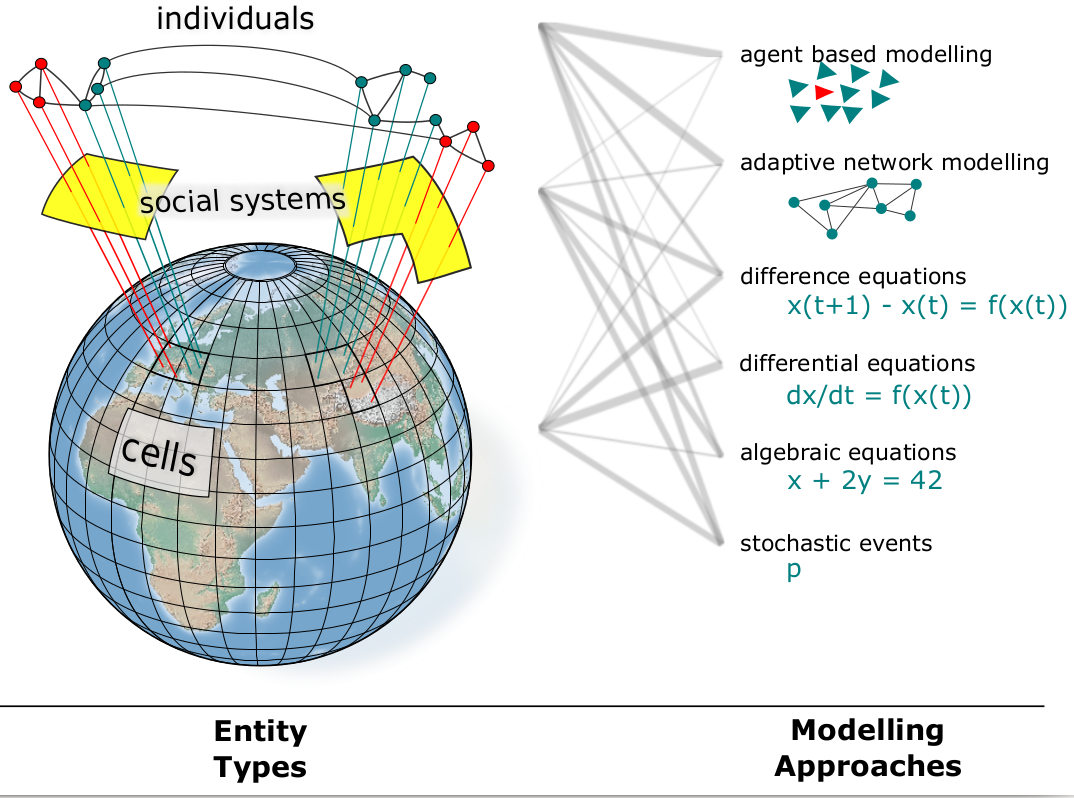
\includegraphics[width = .8 \textwidth]{figures/CORE.png}
  \caption[Illustration of the copan:CORE modeling framework]{\textbf{Illustration of the copan:CORE modeling framework.} From [P3]. The framework integrates different modeling approaches to describe different types of entities that are part of a \emph{whole} Earth system. This includes entities and processes on three levels: a physical and biological, a collective e.g., economic, social and cultural and an individual level.}
  \label{fig:Core}
\end{figure}
In \citep{Donges2018} colleagues and I have argued that a truly integrated modeling paradigm is necessary to appropriately understand the functioning of the Earth system in the Anthropocene. As illustrated in fig.~\ref{fig:Core}, the corresponding modeling framework that we call copan:CORE acknowledges the different nature of various natural and social processes that are integral to Earth system dynamics in the Anthropocene and integrates them in one \emph{whole} Earth system model.

In line with this modeling paradigm, I propose a more nuanced description of human individual and social behavior in the context of socio-economic models that enables the portrayal of social dynamics of norm change and opinion formation as well as individual decision making of heterogeneous agents. 
This description builds on two existing strands of research. First, the literature on opinion formation and social learning models and second, the concept of boundedly rational decision making and fast and frugal heuristics. Subsequently, I give a short explanation of both of these approaches and illustrate how I intend to combine them.

\section{Bounded Rationality and Fast and Frugal Heuristics}
\label{sec:intro_bounded_rationality} 
% Modelling societal change: Individual and collective level:
% Make the case for bounded rationality 
Classical models of rational decision theory that are in line with the paradigm of the `homo economicus' and in use in neoclassical economics and beyond define `rationality' as rational choice theory combined with utility maximization and Bayesian probability inference \citep{wilkinson2012introduction} in addition to complete understanding of the surrounding that individuals operate in which enables them to form so called `rational expectations'. 

With respect to these rather strong assumptions about human cognitive capabilities, knowledge and rigor, Herbert A. Simon famously wondered: \\

``How do human beings reason, when the conditions for rationality postulated by the model of neoclassical economic theory are not met?''  \citep{simon1989scientist}\\

Consequently, he started to develop models of human decision making assuming that human beings do not posses the computational powers to perform optimization tasks and therefore must use some different way of reasoning \citep{simon1982models}. He argued that heuristic processes would be suited far better than optimization under constraints to describe human decision making and coined the term `Bounded Rationality' for this science of decision making that was informed by the boundaries and decision problems that real humans face.

Besides the fact that humans do not have the computational capabilities to make formally rational choices in the vast majority of cases, the classical view on rationality has another, even more fundamental problem. This problem lies in the fact that Bayesian methods only yield meaningful results in isolated decision situations, so called `small worlds'. In other words, to apply them, the complexity of the real world has to be reframed and reduced to a small world that consists of a set of possible actions whose consequences are -- at least in principle -- knowable\footnote{The real world has to be formulated in terms of a set of possible states of the world, actions and consequences or outcomes whose distributions depend on a set of parameters. Usually, these parameters are considered to be constant.} \citep[for an elaboration see p. 82 ff.][]{savage1972foundations}. The assumption that is often implicit is that the insights gained from the analysis of this `small world' can then be transferred to the `large world' that was previously abstracted from and yield similar results. However, this assumption has proven to be harmful, e.g., in the 2008 financial crisis in face of which \cite{Stiglitz2010} noted: ``It simply wasn't true that a world with \emph{almost} perfect information was very similar to one in which there was perfect information''. So, even though Bayesian methods are generally proven and tested in theory, it seems not entirely clear whether they can be applied to complex real world problems in this generality.
Similarly, \cite{binmore2008rational} emphasizes that in `large worlds' one can no longer assume that ``rational'' models automatically provide correct answers.\\
Also, there was growing evidence that in certain `large world' situations, simple heuristics that ignored part of the available information performed equally good or better than more complex models such as linear multiple regression \citep{Czerlinski1999} or neural networks trained via back propagation and different decision tree algorithms \citep{Chater2003, Brighton2006}.

With these doubts in mind about Bayesian inference as an all purpose decision framework, \cite{Gigerenzer1996} proposed a different paradigm for human decision making that they call `Fast and Frugal Heuristics'. 
This paradigm tried to understand decision making by learning from flesh and bones decision makers that learned to cope with complex `large world' problems. In their research, they find that such decision makers can learn to use their inability to process all available information to their benefit -- they develop heuristic methods that use the right information in the right way and ignore the rest. They define these heuristics as
\\

``strategies that ignore part of the information, with the goal of making decisions more quickly, frugally, and/or accurately than more complex methods \citep{Gigerenzer2011}.''\footnote{Note that ignoring available information is not unique to this approach. In state-of-the-art machine learning techniques robustness and accuracy can be greatly improved if humans intelligently preselect the variable and features that are used to train a specific model \citep{Guyon2003}.} \\

These heuristics are process-oriented models of human decision making that integrate the search for relevant information as well as their evaluation into simple algorithmic rules. `Process-oriented' means that in contrast to so-called `as if' models that mathematically integrate all available information to mimic human decisions, these models are aligned to the actual process of reasoning. It is also assumed that rather than one multipurpose tool like Bayesian inference, humans carry an `adaptive toolbox' of specialized heuristics \citep{gigerenzer2002bounded} that are used according to the requirements of the actual decision problem.
In fact, certain heuristics work surprisingly well in certain environments and perform equally or even better than more complex and computationally demanding models such as multiple regression or Bayesian inference \citep{Gigerenzer2009}. This property is called \emph{ecological rationality} in the sense that there is not one rational model of reasoning, but rationality lies in the fruitful combination of a specialized method and an environment that fits its capabilities \citep{todd2007environments}.
\begin{wrapfigure}[17]{i}{.3 \textwidth}
  \centering
  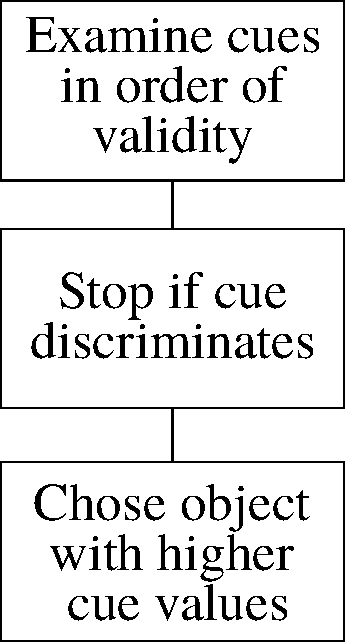
\includegraphics[width = .18 \textwidth]{figures/TTB.pdf}
  \caption{Schematic illustration of the Take The Best heuristic}
  \label{TTB}
\end{wrapfigure}
To point out the nature of this kind of reasoning, these heuristics will be illustrated along the following example: \emph{Take The Best} \citep{Gigerenzer1996} is a heuristic that can be used to decide between two alternatives that can be described by a number of pieces of information, so called cues. As illustrated in figure \ref{TTB} the heuristic evaluates these cues according to a predefined order and makes a decision as soon as the first evaluated cue discriminates between the alternatives, favoring the alternative with the higher (better) cue value. If no cue discriminates, one of the alternatives is chosen at random with equal probabilities. Thereby this heuristic makes inferences based upon only one cue and ignores all others.\footnote{Of course this ignorance of available information only holds for the application of the heuristic where the order in which cues are evaluated is considered to be given. To find the right cue order that matches the structure of the decision environment one has to use all the available information -- but more on that later.} Also, it only relies on simple comparison and does not make any calculations whatsoever.\\
It can easily be generalized to decide between a number of alternatives by simply comparing them cue by cue and ruling out the alternatives with negative cue values.
It is strictly ecologically rational in environments with rapidly decaying cue weights, i.e. where some pieces of information are significantly more important than others. It is worth mentioning that this model successfully explains so called `less is more' effects, where people with little knowledge on a topic are able to make better inferences than those who know more. There is evidence \citep{Garcia-Retamero2009,Pachur2013} that
%For a classification of an object involving $m$ cues, a \textbf{Fast and Frugal Tree} (FFT) \cite{Martignon2008} is a decision tree with $m$ leaves and an exit for the first $m-1$ cues
%\begin{wrapfigure}[20]{i}{.55 \textwidth}
%  \includegraphics[width = .5 \textwidth]{figures/FFT.pdf}
%  \caption{Schematic illustration of a Fast and Frugal Tree as used for medical decision making to classify incoming heart attack patients into high or low risk patients.\label{FFT}}
%\end{wrapfigure}
%and two exits for the last cue. This means that it is composed of sequentially ordered cues and to make a decision it starts by evaluating the objects first cue in this sequence. If this cue meets the respective exit condition, a decision is made and no other cues need to be evaluated. Otherwise the FFT considers the other cues one after another until an exit condition is met. Note that a binary decision problem as treated by the previous heuristics can be framed as a binary classification as well but not vice versa. Also, in addition to a cue order, this heuristic is characterized by an exit structure. This exit structure defines the direction of the leaves of the decision tree for each evaluated cue i.e. whether on each stage of the sequence the compliance with the requirement for the cue leads to a classification in one or the other category or the evaluation of further cues. Speaking in the terminology of signal detection theory, this can be used to tweak the classification process in an either liberal or conservative direction \cite{Luan2011}.\\
%The prevalence and ecological rationality of this kind of heuristic is a question of ongoing research, but they have been tested against medical, judical and financial decisions in different environments \cite{dhami2001bailing,dhami2001fast,keller2014tying} where they accurately predicted doctors, magistrates and investors decisions and they were benchmarked against datasets of military defense decisions where they performed equally good or better then more complex benchmark strategies including logistic regression in prescriptive accuracy. \\ 
expertise in a certain task mainly comes from implementing a suitable heuristic and a decent cue ordering in case this heuristic features one. This means, that besides knowing `what really counts' which is reflected in a cue order that properly accounts for the distributions and validities of information in the respective environment, the way in which this information is looked up and evaluated differs between agents and has significant effect on their performance.

Also, although in a scientific context most decisions scenarios under consideration comprise of inferential choice where decisions can be right and wrong, the same lines of heuristic reasoning work for preferential choice as well. In this case, cue orders do not so much represent knowledge about the significance of pieces of information but rather values, norms or other, underlying, more fundamental preferences.

Finally, as much as an `adaptive toolbox' of heuristics for numerous purposes might be a realistic approach to the human mind dealing with many different environments, this approach raises another question: how does one decide on which heuristic, cue order or decision tree structure to use? Current research \citep{garcia2009does,Rieskamp2006} considers reinforcement learning of decision making agents or different sorts of imitation processes. This is especially interesting because it directly links the adaptation of the decision process to the dynamics of the environment and the social structure in which the decision maker is embedded.\\

% Discuss models of opinion formation and social learning
\section{Opinion formation and Social Learning}
Social learning describes the process of learning new behaviors and information by observing and imitating others \citep{Bandura1971}. 
% historical models for opinion formation and social learning.
Conceptually, such processes were studied with methods from statistical physics since the 1970s \citep[for a review see e.g.][]{castellano2009statistical}. This was done by representing individuals as nodes in a network and their connections or interactions with other individuals as links to other nodes. Individuals' opinions are represented as  variables, i.e. a set of numbers and changes in opinions are described by a set of mathematical rules for the interactions of one or more neighboring nodes. One of the first models that was extensively studied in many variants is the so called `voter model' \citep{Clifford1973, Holley1975}. It is defined by individuals that are represented by nodes in a network who are characterized by a binary opinion variable $o_i = \pm 1$. In each time step, an individual $i$ and one of its neighbors $j$ are selected and individual $i$ takes the opinion of individual $j$. One of the reasons that this model became wildly popular at the time was, that it is analytically solvable in many cases. 
Other models for opinion dynamics and social learning include e.g., the Sznajd model, the Deffuant model and Axelrod model. The Sznajd model \citep{Sznajd-Weron2000} is closely related to the Ising spin lattice model, in the Deffuant model \citep{Deffuant2000} randomly selected individuals interact if their difference in opinions is below a certain threshold $|o_i - o_j| < \varepsilon$ in which case their opinions move closer together and in the Axelrod model \citep{Axelrod1997} individuals are characterized by a vector of traits and their interaction probability increases with their overlap in these traits. However, as the network topology of these models is fixed, the analysis is mostly confined to the analysis of the convergence times to one of the absorbing states of the model where only one of the initially prevalent opinions remains.\\
In the early 2000s interest increased in possible effects arising from the simultaneous dynamics \emph{of} and \emph{on} networks \citep[for a review see][]{Gross2008}. In the context of opinion formation and social learning enables the coevolution of the state of individuals and the networked connections between them.\\

The extension of the `voter model' that includes network adaptation is called the `adaptive voter model' \citep{Holme2006a, Bohme2011, Rogers2013, Klamser2016, Min2017}. It describes a network consisting of a constant set of $N$ nodes and $K$ bidirectional links. The nodes represent individuals that have one of $O$ opinions $o_i$. Nodes become active with a constant rate $\frac{1}{\tau}$ such that waiting times between interactions are distributed exponentially. If a node becomes active, it selects one of the nodes from its neighborhood in the network with equal probability. If that node holds the same opinion, nothing happens. If that nodes holds a different opinion, one of two things happens. With probability $\varphi$, the link between the two nodes is removed and the active node selects one node from the previously unconnected nodes that hold the same opinion with equal probability and forms a new link with it.
Contrasting to simple voter models, different variants of the adaptive voter model show interesting phase transitions between absorbing states exhibiting a completely connected network between individuals and absorbing states with a fragmented network topology.

\section{Social Learning of Ecologically Rational Decision Heuristics}
\label{sec:intro_learning_heuristics}

Previously, models of social learning such as the adaptive voter model have been used to describe the spreading of successful behaviors in social ecological systems modeling. For instance \cite{Wiedermann2015}, \cite{Barfuss2017} and \cite{Geier2019} where individuals learned to use high or low harvesting efforts in interacting with a renewable resource. This approach is highly interesting as it is able to describe the qualitative dynamical and structural properties of social dynamics that are essential to modeling sustainability transitions as argued by \cite{Lade2017}.
However, in its current form this approach models social learning and information propagation on networks together with individual agent decision making that determines their actions as one and the same process. Thereby it intrinsically links the actions of agents with the traits that are propagated in the adaptive network process. Thus, it prevents agents from changing their actions independently due to, e.g., information from their ecological environment, changing economic conditions or other information that becomes available to them. 

But, given that I am interested in societal change that is driven by both, social dynamics and individual decision making, I argue that it is productive to model these processes separately. So, \emph{I propose to use adaptive network processes to model the social propagation of ecologically rational decision heuristics}.
I argue that this can be motivated both in inferential and preferential decisions. For inferential decisions, others have argued that humans imitate successful strategies through interaction and imitation \citep{Bandura1971, Traulsen2010} and that these strategies can be the structure of a decision heuristic that fits the environment \citep{Garcia-Retamero2009}. Also, given that according to \cite{Weber2009} and \cite{Gigerenzer2011} preferential and inferential decisions draw on the same processes, it makes sense to model them in the same framework. 

Additionally, I argue that in the case of preferential decisions one can sensibly interpret the internal structure of heuristic decision algorithms such as cue orders or tree structures as norms or preferences that drive an agent's actions and that it is consistent to model their dynamics with the tools that are used to model the spread of norms on social networks.

I present two such models that combine social learning and heuristic decision making with more conventional models of economic dynamics in chapter \ref{chapter:heuristics} and \ref{chapter:savings} and illustrate what kind of questions they may help to answer and what kind of interesting dynamics they can exhibit.

\section{Approximations of Heterogeneous Agent Models}

The complexity of behavioral rules such as the ones that I propose above make an analytic treatment very difficult. Therefore, they are usually analyzed numerically. However, because the model mechanisms are difficult to trace in the black box of a computational model, the results are often difficult to interpret and cannot provide mathematically sound proofs of relationships between model variables. Results may therefore be hard to generalize. Given these shortcomings, it becomes better understandable that there is an apparent preference in mainstream economics that favors deterministic models with few variables over high dimensional computational models.

There is, however, a number of approximation approaches for adaptive network models from statistical physics such as the ones applied by \cite{Rogers2013}, \cite{Wiedermann2015} and \cite{Min2017}. However, all of them consider interactions between agents only on an individual level. Contrasting, approximation methods that have been applied to heterogeneous agent models in economics usually rely on mean field approximations e.g. they make use of Master and Fokker-Planck equations \citep{Aoki1998, Aoki2007, DelliGatti2000, DiGuilmi2008, Chiarella2011a, Landini2014}. Such approaches assume that each agent pair interacts with the same probability.

A few also take network structure into account and derive macroscopic quantities that describe the structure of networks \citep[e.g.][]{Alfarano2008a, Lux2016}.
Yet, most of this literature regards either the network between agents or the states of agents as static, implicitly assuming different time scales for dynamics of and processes on the network.
But, as argued above, to adequately understand the properties of social-ecological and socio-economic systems, one has to include dynamical processes and interactions on a structured individual as well as on an aggregated global level.

In chapter \ref{chapter:approximation} I develop and apply an approximation method that uses moment closure, pair approximation and large system limit approximations to derive an aggregate description for a socio-economic model -- a simplification of the model introduced in chapter \ref{chapter:heuristics} -- that combines local interactions on an adaptive network with system-level interactions through markets. 

